\documentclass[twoside,english]{uiofysmaster}
%\bibliography{references}

\usepackage{array}
\usepackage{booktabs}
\usepackage{float}
\usepackage{scrextend}
\usepackage{amsfonts}
\usepackage{amsmath}
\addtokomafont{labelinglabel}{\sffamily}

\setlength{\heavyrulewidth}{1.5pt}
\setlength{\abovetopsep}{4pt}

\begin{document}


\title{The history of master thesises and other random gibberish}
\author{Ingrid Holm}
\date{September 2017}

\maketitle

\begin{abstract}
This is an abstract text.
\end{abstract}

\begin{dedication}
  To someone
  \\\vspace{12pt}
  This is a dedication to my cat.
\end{dedication}

\begin{acknowledgements}
  I acknowledge my acknowledgements.
\end{acknowledgements}

\tableofcontents




\chapter{Gaussian Processes for Machine Learning}

Gaussian processes are based on the Gaussian distribution of parameters. In Gaussian processes every point in some continuous input space is associated with some normally distributed random variable.

Notes from \cite{rasmussen2006gaussian}. Kernel = covariance function. 

\section{The Linear Bayesian Model}


We divide supervised learning into \textit{regression}, when the output variables are continuous, and \textit{classification}, when output variables are discrete. Assume we have a set of data consisting of input parameters $\textbf{x}$ and output $y$, which we gather in a data set of $n$ points $\mathcal{D}=\{(\textbf{x}_i, y_i)| i=1,...,n\}$. This is the training set, which will be used to train the algorithm. We also have a test set $\textbf{x}_*$, which will be used to test it. In Gaussian Processes a \textit{prior} is made; an assumption of the form of the function $f(x)$. We assume it follows a Gaussian distribution with a \textit{mean} and a \textit{covariance matrix}.

Supposing we have a data set of two points, $\mathcal{D} = \{(\textbf{x}_1,y_1), (\textbf{x}_2,y_2)\}$, there are many functions that could pass through these points. The \textit{mean} of these functions is the one GP chooses. The variance at the data points is small, as can be seen in Fig. (\ref{Fig:: Gaussian function example 2 points}). Combining the prior and the data, gives the \textit{posterior}.


\begin{figure}[H]
\label{Fig:: Gaussian function example 2 points}
\centering
\includegraphics[scale=0.5]{figures_Ingrid/rasmussen_gaussian_example1.png}
\caption{From \cite{rasmussen2006gaussian}: Panel (a) shows four samples drawn from the prior distribution. Panel
(b) shows the situation after two datapoints have been observed. The mean prediction
is shown as the solid line and four samples from the posterior are shown as dashed
lines. In both plots the shaded region denotes twice the standard deviation at each
input value x.}
\end{figure}


The specification of the prior is important, as this encodes the knowlegde we have about the functions. It can for example be stationary, meaning that the different functions behave similarly at the same $x$-values. This type of characteristic is encoded in the \textit{covariance function}, which tells us something about the correlation between points (or in this case functions). In Gaussian processes the consept of learning means finding the best fit for the components of the covariance function.

The training set consists of $D$-dimensional vectors features $\textbf{x}$, which we gather in the \textit{design matrix} $X$, and targets $y$, which we gather in an $n$-dimensional vector $\textbf{y}$.

We denote the \textit{Gaussian distribution} with mean $\mu$ and variance $\sigma^2$ as $\mathcal{N}(\mu, \sigma^2)$. A random variable distributed according to the Gaussian, or normal, distribution is denoted as $X \sim \mathcal{N}(\mu, \sigma^2)$. A general Gaussian distribution is given by
\begin{align}\label{Eq:: General Gaussian Distribution}
f(x|\mu, \sigma^2) = \frac{1}{\sqrt{2 \pi} \sigma} e^{-\frac{1}{2} (\frac{x-\mu}{\sigma})^2}.
\end{align}
A Bayesian analysis of a linear model with Gaussian noise requires an input vector $\textbf{x}$, a vector of weights $\textbf{w}$, a function value $f$ and an observed target value $y$. We also get a noise parameter $\epsilon$ that follows a Gaussian distribution
\begin{align}\label{Eq:: Gaussian dist noise}
\epsilon \sim \mathcal{N}(0, \sigma_n^2).
\end{align}
We then have the following relations
\begin{align}\label{Eq:: Gaussian linear w noise}
f(\textbf{x}) &= \textbf{x}^T \textbf{w}, &y = f(\textbf{x}) + \epsilon.
\end{align}

The probability density of the observations given the parameters is called the \textit{likelihood function}, and is given by
\begin{align}\label{Eq:: Gaussian linear likelihood function}
p(\textbf{y}|X, \textbf{w}) &= \sum_{i=1}^n p(y_i|\textbf{x}_i, \textbf{w}) = \frac{1}{(2 \pi \sigma_n^2)^{n/2}} \exp \Big( - \frac{1}{2 \sigma_n^2} |\textbf{y}-X^T \textbf{w}|^2 \Big) = \mathcal{N}(X^T \textbf{w}, \sigma_n^2I).
\end{align}

For the weights we use a zero mean Gaussian distribution with covariance matrix $\Sigma_p$,
\begin{align}\label{Eq:: Gaussian linear weight dist}
\textbf{w} \sim \mathcal{N} (\boldsymbol{0}, \sum_p).
\end{align}
This is our assumption \textit{prior} to the observations. In order to find the posterior we must combine this with the data, for which we use \textit{Bayes theorem}
\[
 \boxed{\label{Eq:: Bayes theorem}
\text{posterior} = \frac{\text{likelihood} \times \text{prior}}{\text{marginal likelihood}} \Rightarrow p(\textbf{w}|\textbf{y}, X) = \frac{p(\textbf{y}|X, \textbf{w})p(\textbf{w})}{p(\textbf{y}|X)},}
 \]
where the marginal likelihood, used to normalize the expression, is independent of the weights and given by
\begin{align}\label{Eq:: Marginal likelihood}
p(\textbf{y}|X) = \int p(\textbf{y}|X, \textbf{w}) p(\textbf{w}) d \textbf{w}.
\end{align}

Through some calculation (see \cite{rasmussen2006gaussian} Eq. (2.7)) we find that the posterior follows a Gaussian distribution
\begin{align}
p(\textbf{w}|X, \textbf{y}) \sim \mathcal{N} (\bar{\textbf{w}} = \frac{1}{\sigma_n^2} A^{-1} X \textbf{y}, A^{-1}),
\end{align}
where $A = \sigma_n^{-1}XX^T + \Sigma_p^{-1}$. We wish to use the posterior to make predictions for the \textit{target}, or test data, $f_* \equiv f(\textbf{x}_*)$. This is found by averaging the the output of all possible linear models w.r.t the Gaussian posterior
\begin{align}\label{Eq:: Gaussian linear prediction}
p(f_*|\textbf{x}_*, X, y) = \int p (f_*|\textbf{x}_*, \textbf{w})p(\textbf{w}|X, \textbf{y}) d \textbf{w},
\end{align}
which corresponds to a Gaussian distribution
\begin{align}\label{Eq:: Gaussian linear prediction dist}
f_* \sim \mathcal{N} (\frac{1}{\sigma_n^2} \textbf{x}_*^T A^{-1}X \textbf{y}, \textbf{x}_*^T A^{-1} \textbf{x}_*).
\end{align}

If the input data is difficult to fit, it can be projected onto a \textit{feature space} were the linear model is then applied. INtroduce a function $\boldsymbol{\phi} (\textbf{x})$ which maps a $D$-dimensional input vector $\textbf{x}$ into an $N$-dimensional feature space. Then 
\begin{align}\label{Eq:: Gaussian linear feature space}
f(\textbf{x}) = \boldsymbol{\phi}(\textbf{x})^T \textbf{w},
\end{align}
where $\textbf{w}$ is now an $N$-dimensional vector. The predictive distribution is then 
\begin{align}\label{Eq:: Gaussian linear feature posterior dist}
f_*|\textbf{x}_*, X, \textbf{y} &\sim \mathcal{N}(\boldsymbol{\phi}_*^T \Sigma_p \boldsymbol{\Phi}(\textbf{K}+ \sigma_n^2I)^{-1} \textbf{y},\boldsymbol{\phi}_*^T \Sigma_p \boldsymbol{\phi}_* - \boldsymbol{\phi}_*^T \Sigma_p \boldsymbol{\phi}_* - \boldsymbol{\phi}_*^T \Sigma_p \boldsymbol{\Phi}(\textbf{K}+ \sigma_n^2I)^{-1} \boldsymbol{\Phi}^T \Sigma_p \boldsymbol{\phi}_*),
\end{align}
where $\boldsymbol{\phi}(\textbf{x}_*)=\boldsymbol{\phi}_*$ and $K=\boldsymbol{\phi}^T \Sigma_p \boldsymbol{\phi}$. We note that the feature space always enters in the form of
\begin{align}\label{Eq:: form of feature space}
\boldsymbol{\Phi}^T \Sigma_p \boldsymbol{\Phi} \text{, } \boldsymbol{\Phi}_*^T \Sigma_p \boldsymbol{\Phi} \text{, or } \boldsymbol{\Phi}_*^T \Sigma_p \boldsymbol{\Phi}_*,
\end{align}
so we we define the \textit{kernel} or \textit{covariance function}
\begin{align}\label{Eq:: Gaussian linear kernel}
k(\textbf{x}, \textbf{x}') = \boldsymbol{\Phi}^T \Sigma_p \boldsymbol{\Phi'},
\end{align}
where \textbf{x} and \textbf{x}' are either the training or test sets. Replacing all occurences of the inner products (\ref{Eq:: form of feature space}) by the kernel is called the \textit{kernel trick}.

\subsection{Function-space view}

An example of a covariance function is the \textit{squared exponential} (SE) covariance function. The covariance between random variables is then 
\begin{align}\label{Eq:: squared exponential cov func}
\text{cov} \big(f(\textbf{x}_p), f(\textbf{x}_q) \big) = k(\textbf{x}_p, \textbf{x}_q) = \exp \Big(- \frac{1}{2} \frac{|\textbf{x}_p - \textbf{x}_q|}{\ell^2}^2 \Big).
\end{align}
So the covariance between nearby points is high. In fact, we've introduced what we call the \textit{characteristic length scale} $\ell$, which we can view as "roughly the distance you have to move in input space before the function value can change significantly" \cite{rasmussen2006gaussian}.

We introduce the \textit{marginal likelihood}, defined as
\begin{align}\label{Eq:: Marginal likelihood}
p(\textbf{y}|X) = \int p (\textbf{y}|\textbf{f}, X) p (\textbf{f}|X)d \textbf{f},
\end{align}
and the \textit{log marginal likelihood}
\begin{align}\label{Eq:: Log marginal likelihood}
\log p(\textbf{y}|X) = - \frac{1}{2} \textbf{y}^T (K+ \sigma_n^2I)^{-1} \textbf{y} - \frac{1}{2} \log |K+ \sigma_n^2 I | - \frac{n}{2} \log 2 \pi.
\end{align}
An example of an algorithm that implements GPs uses \textit{Cholesky decomposition}
\begin{itemize}
\item $L := \text{cholesky}(K+\sigma_n^2 I)$
\item $\boldsymbol{\alpha} := L^T \setminus (L\setminus \textbf{y})$
\item $\bar{f}_* := \textbf{k}_*^T \boldsymbol{\alpha}$
\item $\textbf{v} := L\setminus \textbf{k}_*$
\item $\mathbb{V}[f_*] := k(\textbf{x}_*,\textbf{x}_*) - \textbf{v}^T \textbf{v}$
\item $\log p(\textbf{y}|X) := - \frac{1}{2}\textbf{y}^T \boldsymbol{\alpha} - \sum_i \log L_{ii} - \frac{n}{2} \log 2 \pi$
\item \textbf{return}: $f_*$ (mean), $\mathbb{V}[f_*]$ (variance), $\log p(\textbf{y}|X)$ (log marginal likelihood).
\end{itemize}

Recall that the covariance function has parameters such as $\ell$ and $\sigma_n^2$ which can be adjusted. e call such parameters \textit{hyperparameters}. 

\subsection{Evaluating the result}

In order to evaluate the resulting prediction at each point we introduce the \textit{loss function} $\mathcal{L}$. This specifies the loss when choosing the value $y_{guess}$ when the true value is $y_{true}$. Since the true value is not known, we can instead use the expected loss, and try to minimize this 
\begin{align}
\tilde{R}_{\mathcal{L}} (y_{guess}|\textbf{x}_*) &= \int \mathcal{L}(y_*,y_{guess})p(y_*|\textbf{x}_*, \mathcal{D})dy_*,\\
y_{optimal}|\textbf{x}_* = \text{argmin} \tilde{R}_{\mathcal{L}} (y_{guess}|\textbf{x}_*).
\end{align}

\textit{Stationary} kernels, or covariance functions, depend only on the distance between points, and are independent of their absolute values. \textit{Non-stationary } kernels depend on the absolute values of the points. Stationary kernels are therefore invariant under translations in input space. 















\chapter{Distributed Gaussian Processes}

This is based on the article by Deisenroth and Ng \cite{deisenroth2015distributed}. The main point of Distributed Gaussian Processes is to divide the data set into subsets, and use a Product-of-experts method to reduce the computational cost. Consider a Gaussian Process (GP) with a training set $\mathcal{D}$, which we partition into subsets $\mathcal{D}^{(k)} = \{ \textbf{X}^{(k)}, \textbf{y}^{(k)}\}, k=1,...,M$. Each of these subsets gets a GP. Several nodes are then combined into parent nodes recursively until we get a multi-layered tree structure computational graph, see Fig. (\ref{Fig:: DGP leaf nodes}). 

\begin{figure}[H]\label{Fig:: DGP leaf nodes}
\centering
\includegraphics[scale=0.35]{figures_Ingrid/DGP_leaf_nodes.png}
\caption{From \cite{deisenroth2015distributed}: Computational graphs of hierarchical PoE models. Main computations are at the leaf nodes (GP experts, black). All other
nodes recombine computations from their direct children. The top node (blue) computes the overall prediction.}
\end{figure}

The marginal likelihood $p(\textbf{y}|\textbf{X}, \boldsymbol{\theta})$ factorizes into the product of the $M$ separate terms,
\begin{align}\label{Eq:: DGP marginal likelihood}
p(\textbf{y}|\textbf{X}, \boldsymbol{\theta}) \approx \prod_{k=1}^M p_k (\textbf{y}^{(k)}|\textbf{X}^{(k)}, \boldsymbol{\theta}).
\end{align}

We want the hyper-parameters $\boldsymbol{\theta}$ that maximize the log-marginal likelihood
\begin{align}\label{Eq:: DGP log-marginal likelihood}
\log p(\textbf{y}|\textbf{X}, \boldsymbol{\theta}) &\approx \sum_{k=1}^M \log p_k (\textbf{y}^{(k)}|\textbf{X}^{(k)}, \boldsymbol{\theta}),\\
\log p (\textbf{y}^{(k)}| \textbf{X}^{(k)}, \boldsymbol{\theta}) &= - \frac{1}{2} \textbf{y}^{(k)} (\textbf{K}_{\psi}^{(k)} + \sigma_{\epsilon}^2 \textbf{I})^{-1} \textbf{y}^{(k)} - \frac{1}{2} \log |\textbf{K}_{\psi}^{(k)} + \sigma_{\epsilon}^2 \textbf{I})| + \text{const.},
\end{align}
where $\textbf{K}_{\psi}^{(k)}= k(\textbf{X}^{(k)}, \textbf{X}^{(k)})$ is an $n_k \times n_k$ matrix, and $n_k \ll N$ is the size of the data set for the $k$th expert. Computing the inverse and determinant of $\textbf{K}_{\psi}^{(k)} + \sigma_{\epsilon}^2 \textbf{I}$ requires $\mathcal{O}(n_k^3)$ time with standard implementation.













\chapter{Supersymmetry}

\section{NLO-terms}














\chapter{Logg for GP.py}
\section{Before running on Abel}
$\tilde{c}_L \tilde{c}_L$: Tried BDT.py and GP.py for $m_{2R}$, $m_{2L}$ and $m_{\tilde{g}}$. BDTs worked fine, but GPs got an unexpected peak at 1, and very large errors. Removing the superfluous mass (checked relevance with BDT script), centered the histogram around $0$. \textbf{Are Gaussian processes very sensitive to non-relevant parameters?} 

\begin{table}[H]
\begin{tabular}{|r|c|c|c|c|c|c|c|c|}
\hline
Number & -4 & -3 & -2 & -1 & 1 & 2 & 3 & 4\\
\hline
Squark & $\tilde{c}_L$ & $\tilde{s}_L$ & $\tilde{d}_L$ & $\tilde{u}_L$ & $\tilde{u}_R$ & $\tilde{d}_R$ & $\tilde{s}_R$ & $\tilde{c}_R$\\
\hline
\end{tabular}
\end{table}

Running on Abel with $normalize_y=True$ for training data $0,001$, $0,1$ and $0,8$ (where $1=100\%=10 000$ points).


\chapter{Abel}
Running with $normalize_y=True$ with normal Gaussian processes.
\begin{table}[H]
\centering
\begin{tabular}{|c|c|}
\hline
Number of points & Time (hh.mm.ss)\\
\hline
100 & 00:00:23\\
1000 & 00:01:30\\
8000 & 03:40:12\\
\hline
\end{tabular}
\caption{Running times for running $GP.py$ on the Abel supercomputer, with normalize y= True for $n=0.001,0.1,0.8$.}
\end{table}

The histogram of errors from running with 8000 training points can be found in Fig. (\ref{Fig:: Abel 8000p error hist}).

\begin{figure}[H]
\centering
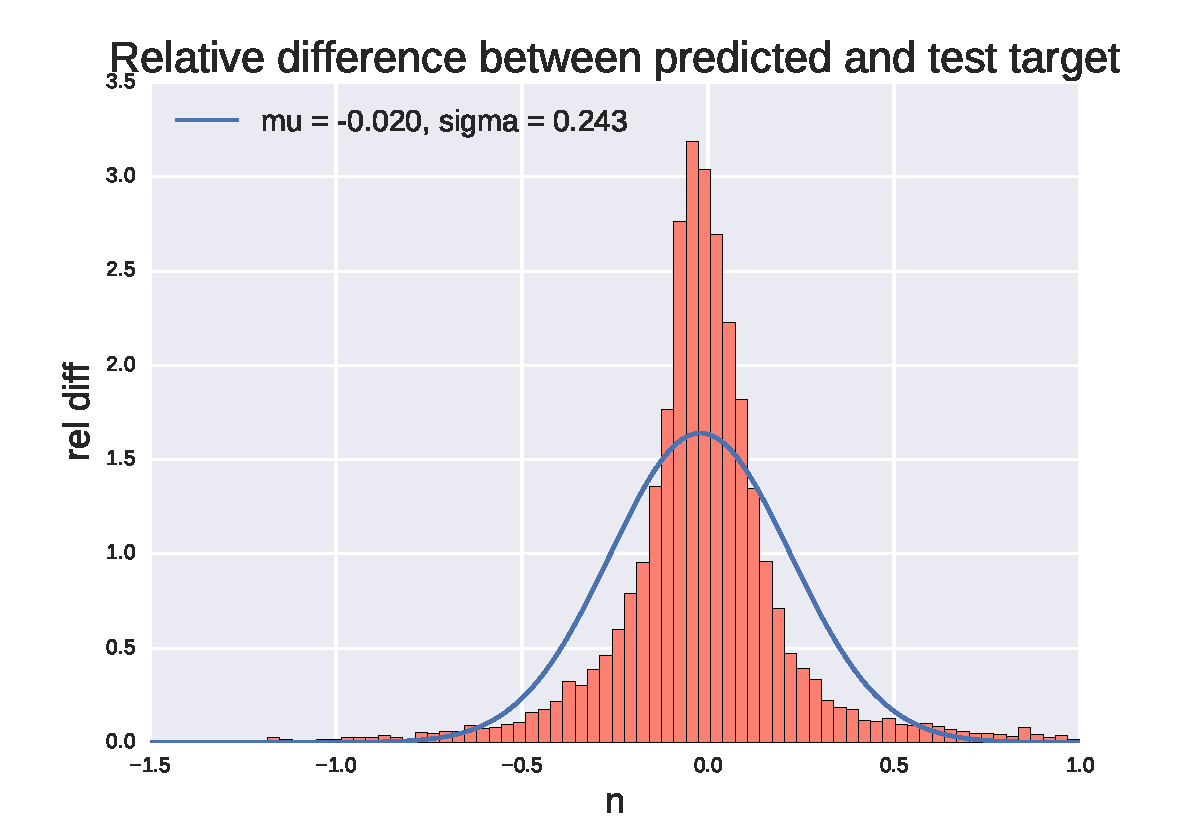
\includegraphics[scale=0.5]{/home/ingrid/Documents/Master/ML/Abel_lin_10000/Plots/meanerror_gaussian_fit.pdf}
\caption{Normalized histogram of relative errors $(y_{true} - y_{predict})/y_{true}$ for 8000 training points run on Abel supercluster. Input parameters are $m_{\tilde{g}}$ and $m_{\tilde{c}_L}$. A Gaussian curve has been fitted using $scipy.stats.norm$.}
\label{Fig:: Abel 8000p error hist}
\end{figure}


The data was split according to the $\log$ of the NLO cross section term, and Gaussian distribution fits were found for each interval. Histograms for $\log= [-25, 2]$ are found in Fig. (\ref{Fig:: Abel 8000p error hist split all}).

\begin{figure}[H]
\centering
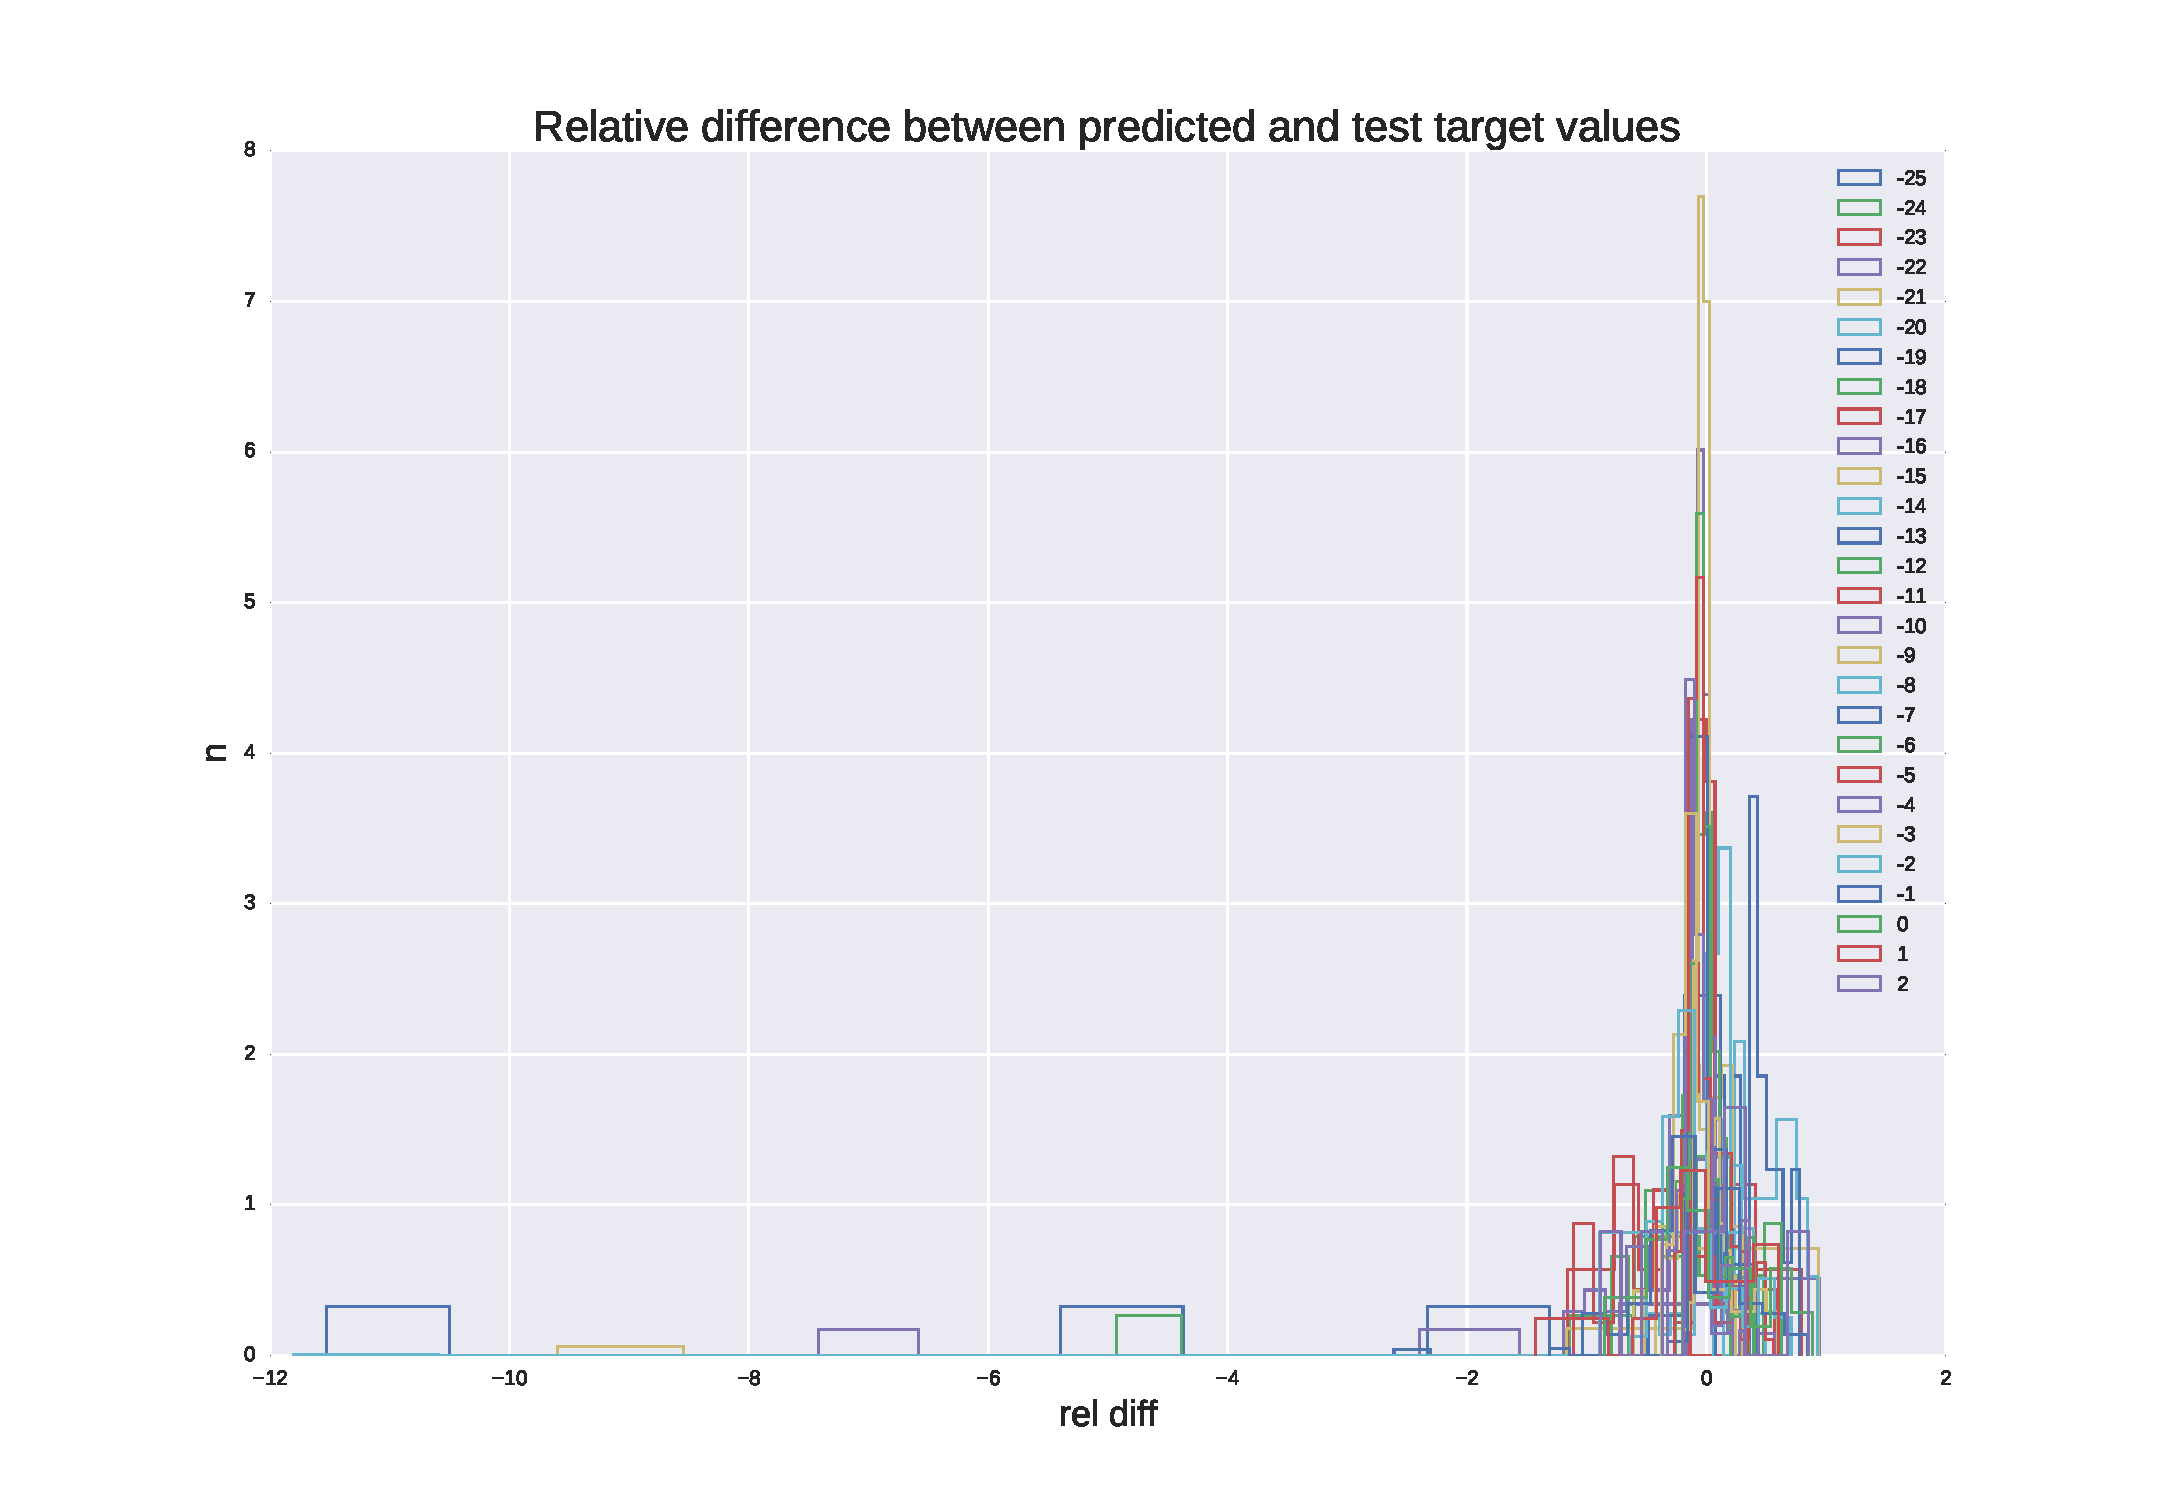
\includegraphics[scale=0.4]{/home/ingrid/Documents/Master/ML/Abel_lin_10000/Plots/test_split_hist_Abel_8000p_all.pdf}
\caption{Normalized histograms for $\log$ of NLO cross section in the interval $[-25,2]$, for 8000 training points run on Abel supercluster. Input parameters are $m_{\tilde{g}}$ and $m_{\tilde{c}_L}$. Gaussian curves were fitted using $scipy.stats.norm$.}
\label{Fig:: Abel 8000p error hist split all}
\end{figure}

\begin{figure}
\centering
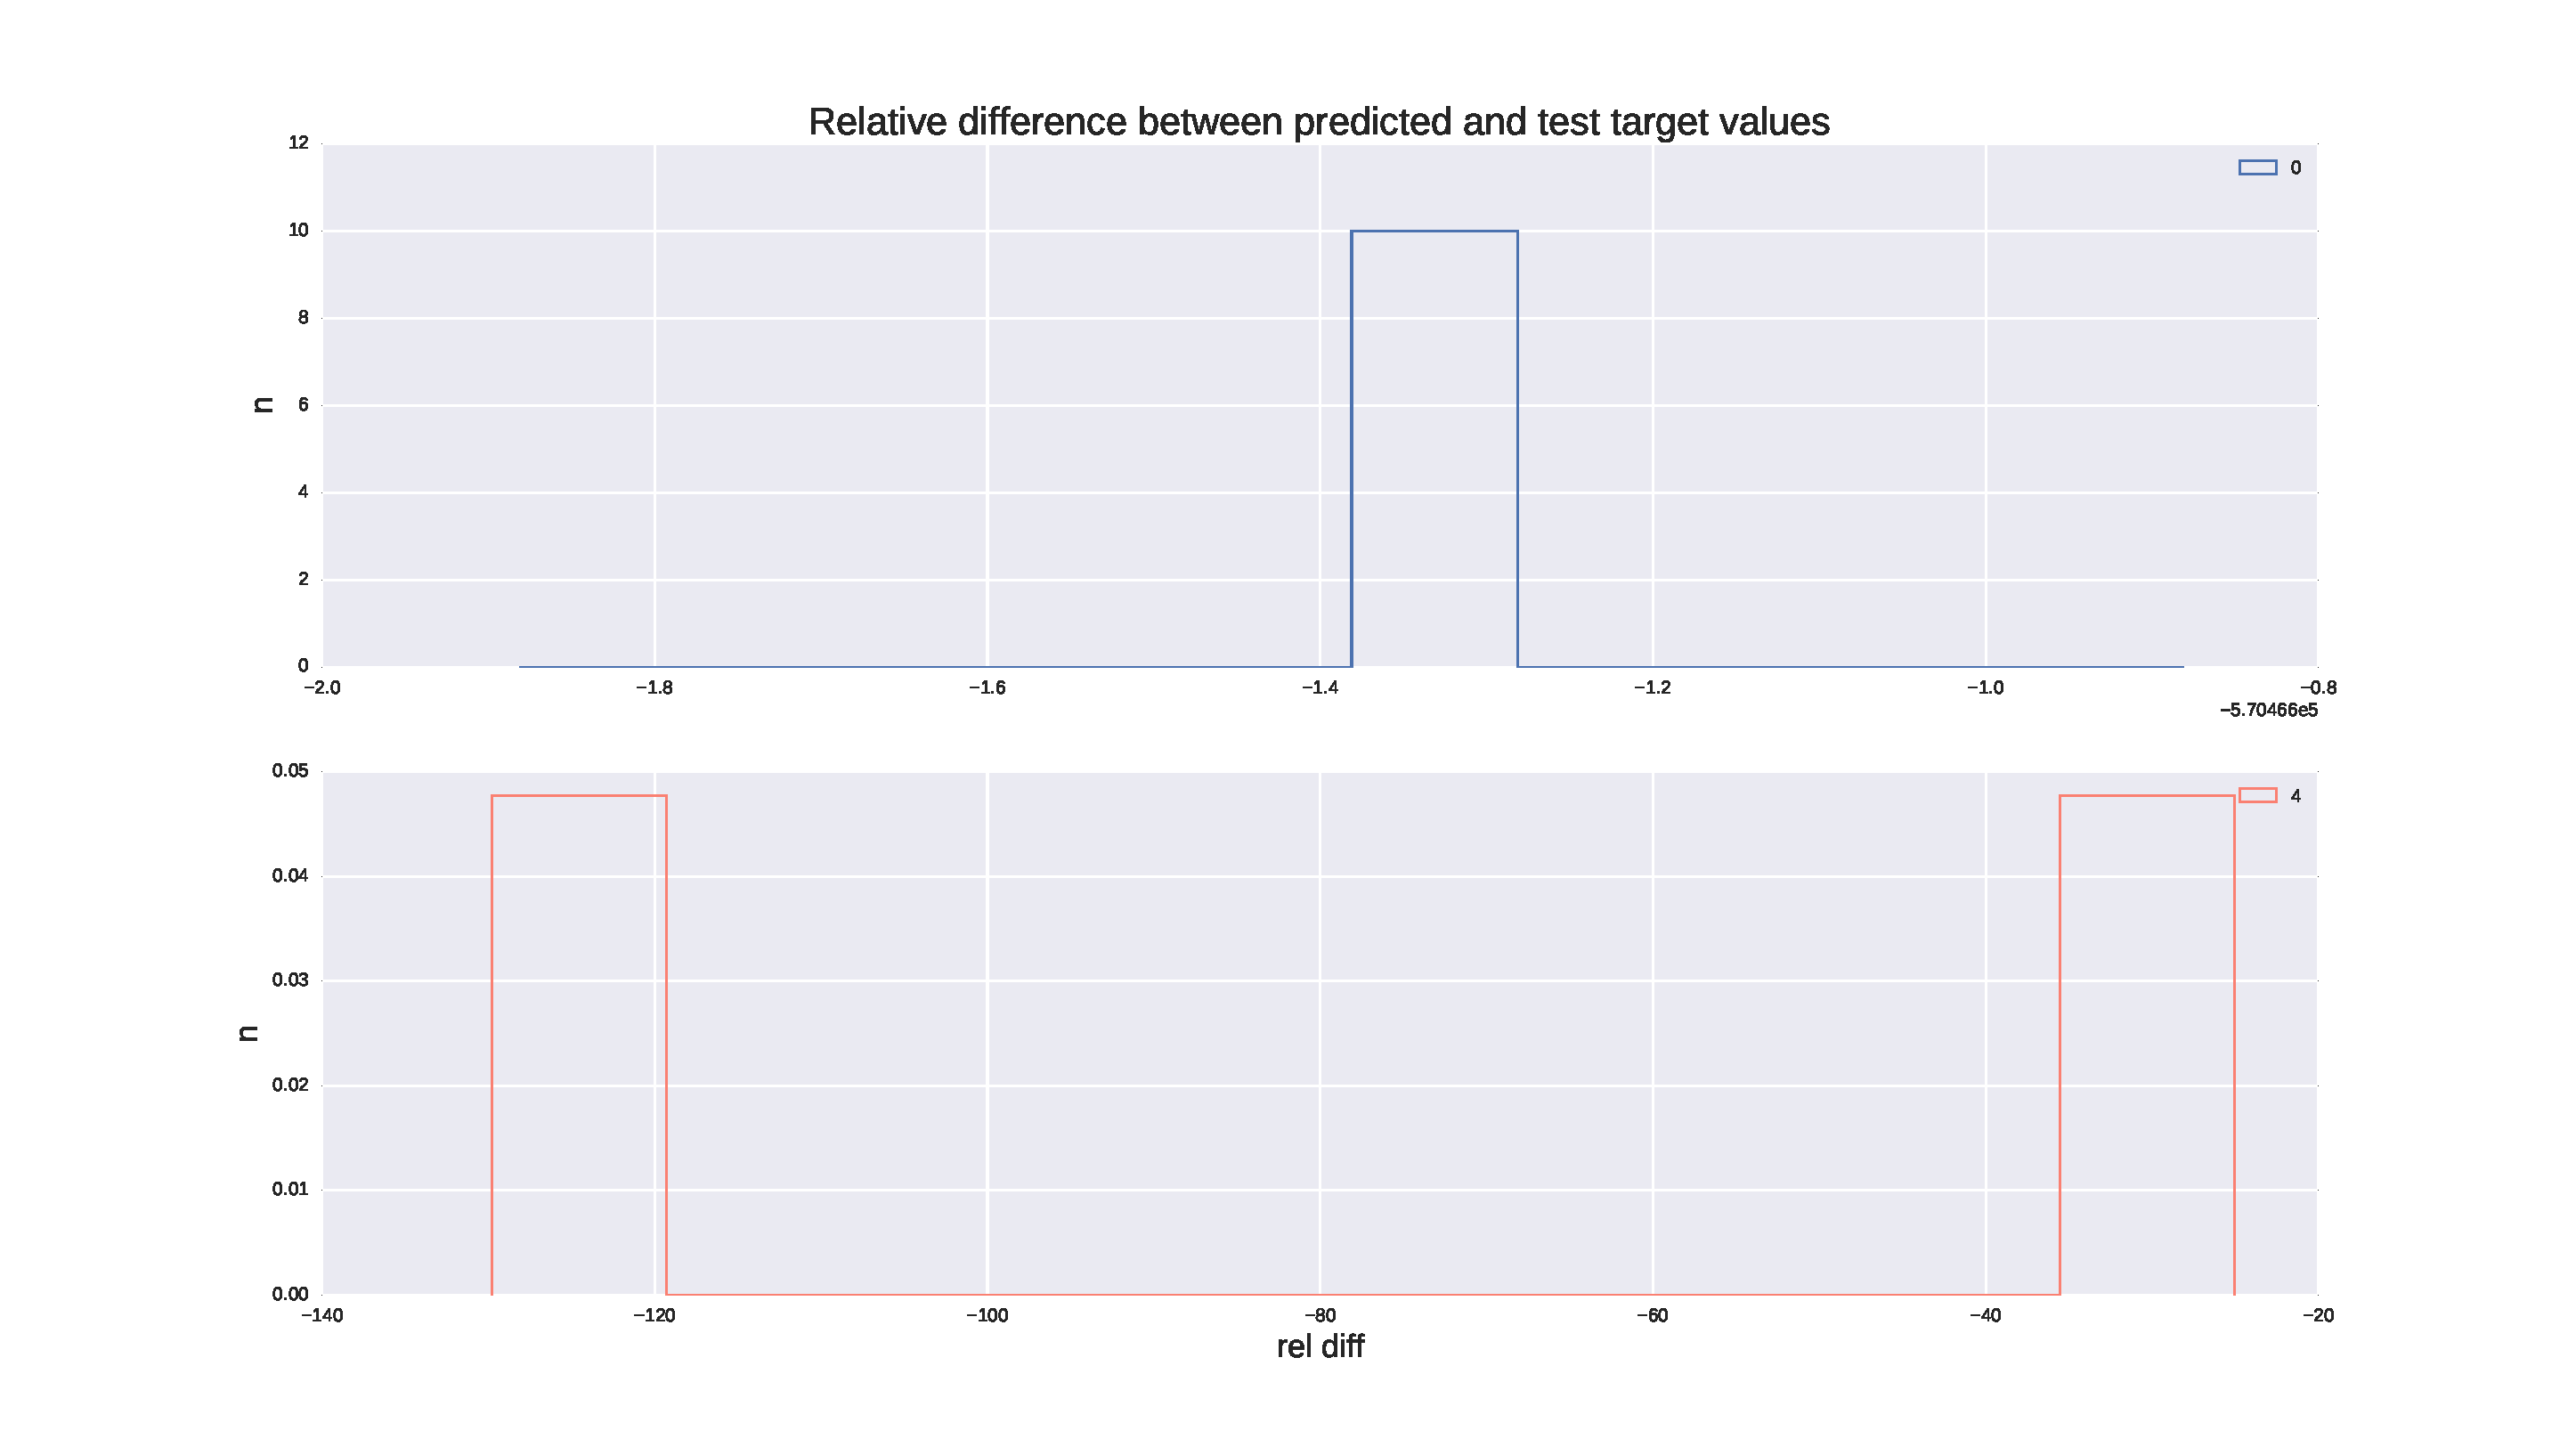
\includegraphics[scale=0.3]{/home/ingrid/Documents/Master/ML/Abel_lin_10000/Plots/test_split_hist_Abel_8000p_weird.pdf}
\caption{Normalized histograms for $\log=0,4$ of NLO cross section, for 8000 training points run on Abel supercluster. Input parameters are $m_{\tilde{g}}$ and $m_{\tilde{c}_L}$. Gaussian curves were fitted using $scipy.stats.norm$.}
\label{Fig:: Abel 8000p error hist split weird}
\end{figure}

The Gaussian fitted parameters are plotted as a function of $\log$ for all values (Fig. (\ref{Fig:: Abel 8000p error hist gauss fit all})) and for $\log= [-25, 2]$ (Fig.(\ref{Fig:: Abel 8000p error hist gauss fit interesting})).

\begin{figure}[H]
\centering
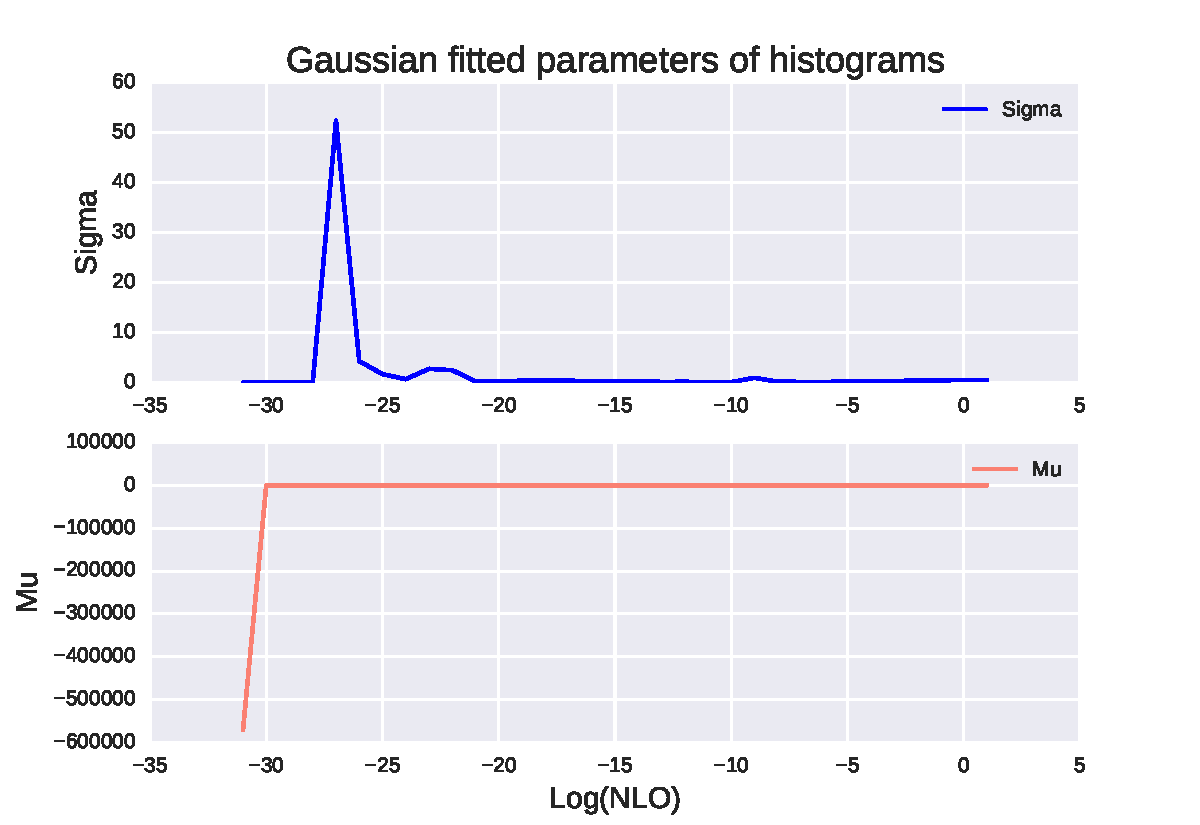
\includegraphics[scale=0.5]{/home/ingrid/Documents/Master/ML/Abel_lin_10000/Plots/test_split_gaussfit_Abel_8000p_all.pdf}
\caption{Gaussian fit parameters as a function of $\log (NLO)$ for all values. 8000 training points run on Abel supercluster. Input parameters are $m_{\tilde{g}}$ and $m_{\tilde{c}_L}$. Gaussian curves were fitted using $scipy.stats.norm$.}
\label{Fig:: Abel 8000p error hist gauss fit all}
\end{figure}

\begin{figure}[H]
\centering
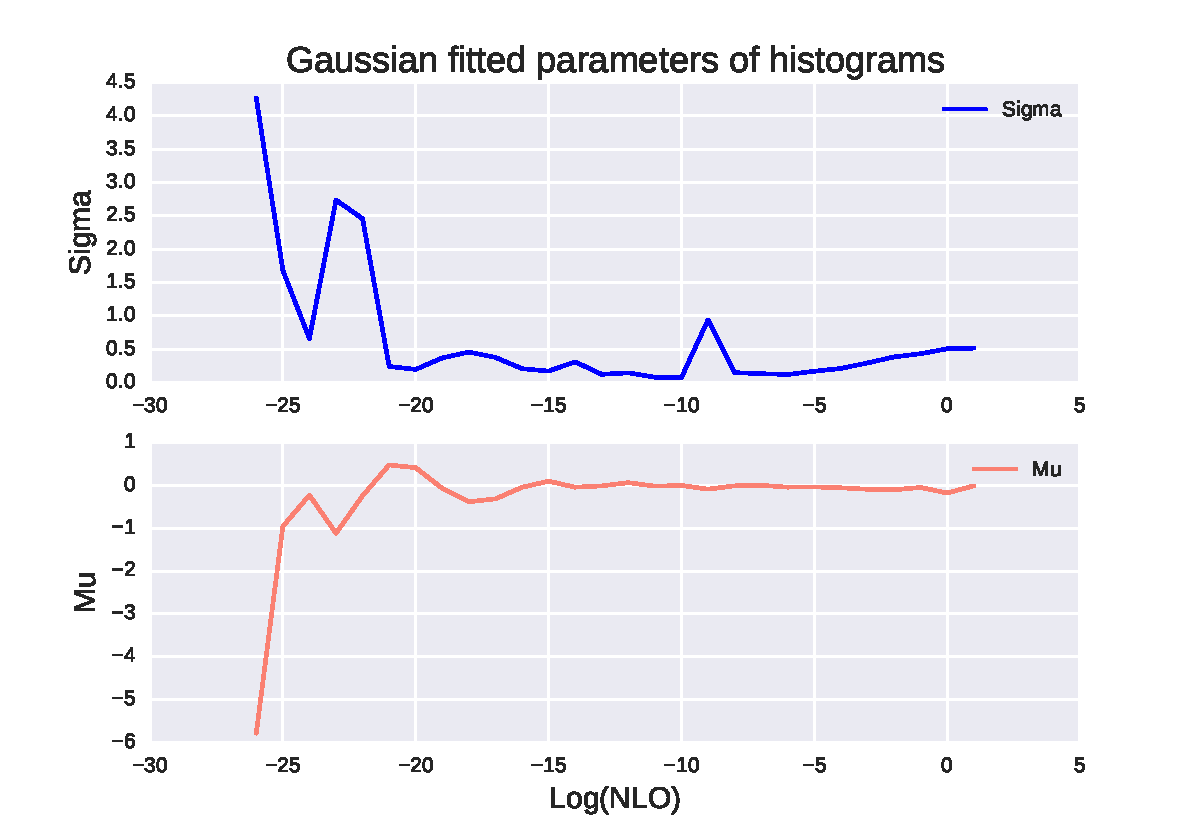
\includegraphics[scale=0.5]{/home/ingrid/Documents/Master/ML/Abel_lin_10000/Plots/test_split_gaussfit_Abel_8000p_interest.pdf}
\caption{Gaussian fit parameters as a function of $\log (NLO)$ for values $\log(NLO) = [-25, 2]$. 8000 training points run on Abel supercluster. Input parameters are $m_{\tilde{g}}$ and $m_{\tilde{c}_L}$. Gaussian curves were fitted using $scipy.stats.norm$.}
\label{Fig:: Abel 8000p error hist gauss fit interesting}
\end{figure}



Divided histograms into intervals of $5$, results are shown in Fig. (\ref{Fig:: Abel 8000p error hist divided}).

\begin{figure}
\centering
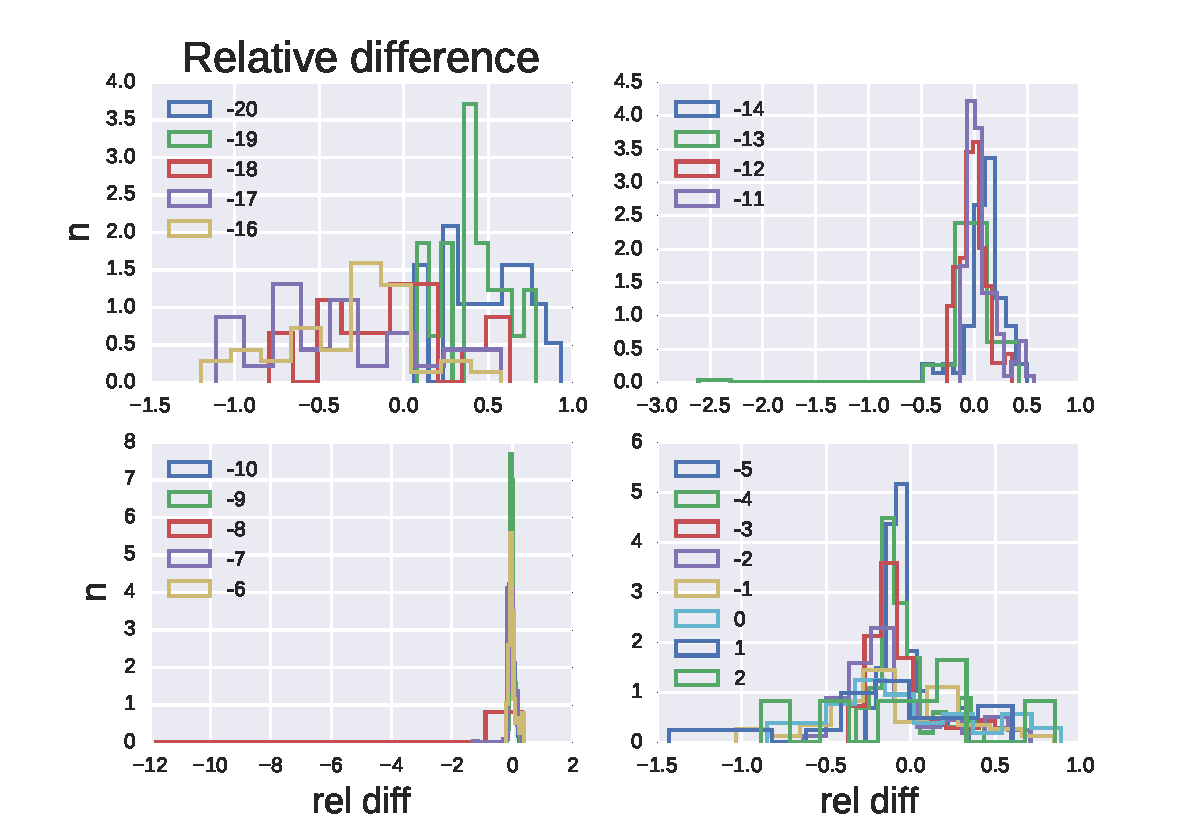
\includegraphics[scale=0.5]{/home/ingrid/Documents/Master/ML/Abel_lin_10000/Plots/test_split_error_hist_Abel_8000p_comparted.pdf}
\caption{Histograms for decades of $\log (NLO)$. 8000 training points run on Abel supercluster. Input parameters are $m_{\tilde{g}}$ and $m_{\tilde{c}_L}$.}
\label{Fig:: Abel 8000p error hist divided}
\end{figure}

OBS! NLO cross sections calculated in Prospino have dimension pb (picobarn) at 8 TeV.

\begin{figure}
\centering
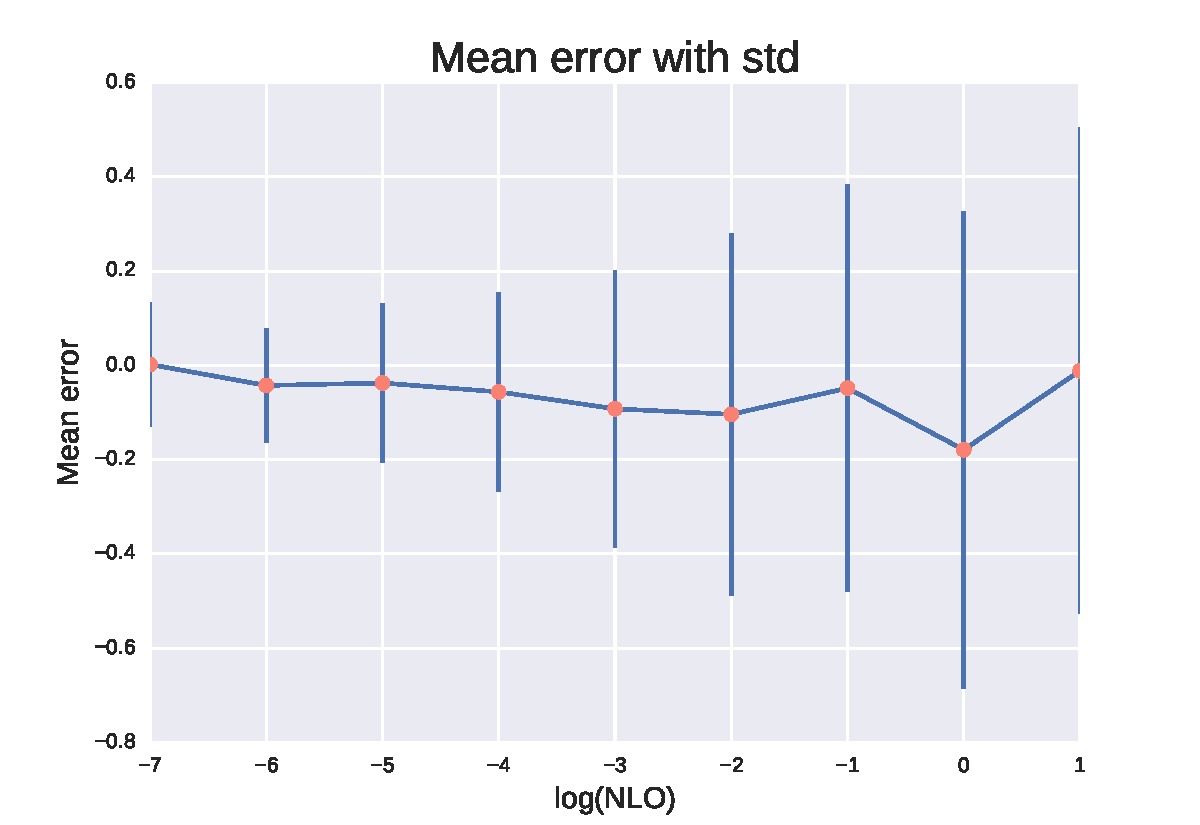
\includegraphics[scale=0.5]{/home/ingrid/Documents/Master/ML/Abel_lin_10000/Plots/Abel_8000p_meanerror.pdf}
\caption{Mean error with standard deviation as a function of $\log (NLO)$. Values less than $-7$ are not considered, as the luminosity at the LHC is $30$ fb$^{-1}$, and so smaller cross sections give $<1$ detectable particles. 8000 training points run on Abel supercluster. Input parameters are $m_{\tilde{g}}$ and $m_{\tilde{c}_L}$.}
\label{Fig:: Abel 8000p mean error with std}
\end{figure}




\section{The curse of dimensionality}














\bibliographystyle{plain}
\bibliography{master_thesis}


\end{document}